\chapter{Compression}
In this chapter we will consider how to compress documents, that deal the problem to reduce 
the amount of data that are travel across network.

Snappy is a compression/decompression library that implement it, usable with several language and 
Google has implement recently \emph{Brotli}, a new compression algorithm for internet.

\section{LZ77 Compression Method}
LZ77 is a compression method, where given a input in the form "past\_knowledge|string\_to\_comprex"
so LZ77 start from string\_to\_comprex and using past knowledge we encode the document with triples
of form $<dist, len, next-char>$, that represent the pattern that was founded in previous string and
we advance in string by $len + 1$.\newline
Usually it used a buffer "window" used to find repeted occurencies to compress and has to be 
the same for encoding and decoding.

The decoding operation do the inverse process, so decoder keeps the same dictionary window as
encoder and finds substring $<dist, len, next-char>$ in previously decoded text and 
insert a copy of it.

\begin{esempio}
	Given the document aacaacab | caaaaaaac we compress the document as following
	\[ <6, 3, a>, <3, 4, c> \]
\end{esempio}

\section{Compression and Networking}
Compression is also important in networking, because it helps to make able the sender and receiver
to share more and more data, to reduce battery usage and so on.

There are $2$ standard techniques used to achieve these results:
\begin{description}
	\item [Caching: ] we want to avoid to send the same object again and it only works 
			  if objects are unchanged.

	\item [Compression: ] remove redundancy in trasmitted data, so avoid repeated substring in
	                      trasmitted data and can be extended with history of past trasmission.

\end{description}
These two standard techniques used two types of situation can happen:
\begin{itemize}
	\item Common knowledge between sender and receiver, and it used with unstructured file 
	      using \emph{Delta Compression} (de/compress $f$ given $f'$).
	\item Partial knowledge between sender and receiver, where in unstructured data it is used
	      \emph{File Synchronization} and in record based data we use \emph{set reconciliation}.
\end{itemize}

\section{Z-Delta Compression}
We have two files f\_known (known to both parties) and f\_new (is known only to the sender) and
the goal is to compute a file f\_d of minimum size such that f new can be derived by the receiver
from f\_known and f\_d; it assume that block moves and copies are allowed, LZ77 decomprension
scheme provides an efficient, optimal solution, so we only compress f\_new based on f\_known
and we decompress f\_d using f\_known .

An example of Z-delta compression importance comes from Dual proxy architecture:
pair of proxies (client cache + proxy) located on each side of the slow link use a 
proprietary protocol to increase performance and we use zdelta to reduce traffic:
so we restricted the number of pages we have to resend it.

We wish also to compress a group of files F useful on a dynamic collection of web pages, 
back-ups, and so on.\newline
To do it we apply pairwise zdelta: find a good reference for each $f \in F$, we reduce
to the Min Branching problem on DAGs and we build a complete weighted graph $G_F$ ,
where nodes are files and weights are the zdelta-size.

We insert a dummy node connected to all, and weights are gzip-coding so we 
compute the directed spanning tree of min tot cost, covering G’s nodes.

Constructing $G$ is very costly, $n^2$ edge calculations, so we wish to exploit 
some pruning approach, like \emph{shrinkling} to detect similar documents given 
$O(n \log n)$ using min-hashing.

\section{File Synchronization}
In File Synchronization we have a Client request to update an old file, who sends a sketch of
the old one to the server.\newline
Server has these new file but does not know the old file, so it sends an update of f\_old
given its received sketch and f\_new

We will briefly analyze two different approach:
\begin{description}
	\item [rsync: ] file synch tool, distributed with Linux and it is simple, widely used and
	                use single roundtrip.\newline
			It uses $4$-byte rolling hash $+ 2$-byte MD5, gzip for literals,
			choice of block size problematic (default: $max\{700, \sqrt{n}\}$ bytes)
			and also there is a high load on the server.

	\item [zsync: ] minimze server load, where computation are done in Client, and has 
			three communication steps visible in figure \ref{img:zsync}.

			\begin{figure}
				\caption{Zsync Computation steps}
				\label{img:zsync}
				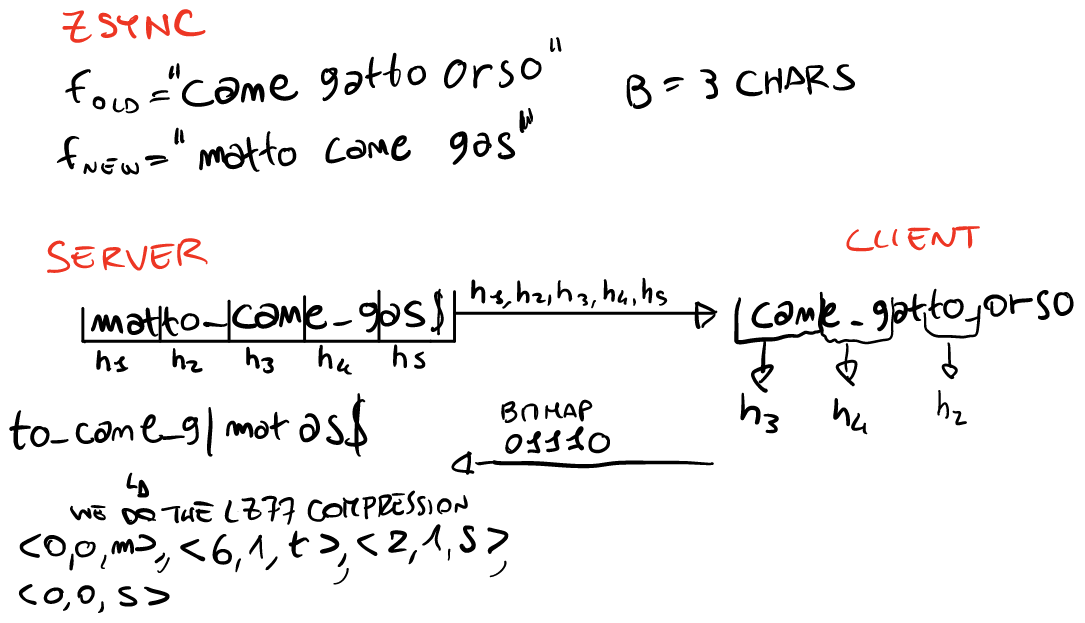
\includegraphics[width=\textwidth]{Images/zsync}
			\end{figure}
			The hashes of the blocks can be precalculated and stored in .zsync file
			and Server should be not overloaded, so it is better suited to 
			distribute multiple-files through network, given one .zsync.

			In our example we have a bitmap of $3$ bits because of \#blocks in
			f\_new are only three.
\end{description}
